\chapter*{Введение}                         % Заголовок
\addcontentsline{toc}{chapter}{Введение}    % Добавляем его в оглавление

Город Москва расширяет свои границы с каждым годом по причине увеличения населения. 
Новому населению требуется жилье. Развитие гражданского строительства достигло поселения 
Сосенское, где в настоящее время возводятся многоэтажные дома и в связи с этим проводятся 
инженерно-геологические исследования площадок для будущего построения жилых 
комплексов. % (Рис. \ref{img:karta}).


%\begin{figure}[ht]
%    \centerfloat{
%      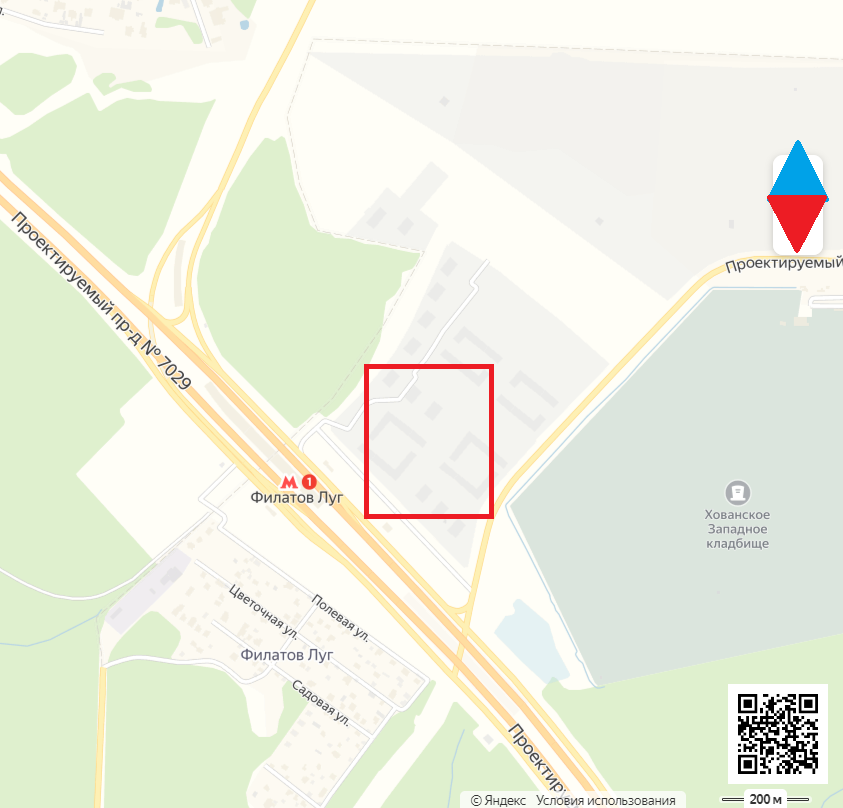
\includegraphics[scale=1]{karta.png}
%    }
%    \caption{Расположение участка исследования}\label{fig:fig}
%  \end{figure}

Поскольку территория изначально не была густо заселена, поэтому требуется более детальная 
изученность инженерно-геологических условий района.

%Исследования проводились проектно-изыскательной компанией ООО~<<ГеоГрадСтрой>>. 
%Было определено геологическое строение района, изучены физические и физико-механические свойства грунтов основания. 
%По предоставленным организацией данным была построена схематическая карта геологического строения.
%
В геологическом прошлом территория города Москвы и район исследования в том числе были 
покрыты ледниковыми покровами. Различают ледники двух эпох "--- московского и донского оледенения. 
Считается, что присутствие ледниковых покровов изменяет напряженно-деформированное состояние 
грунтов, они переуплотняются за счет веса вышележащего ледника, а после его отступления, 
грунты разгружаются. Эти процессы повлияли на настоящие физико-механические свойства грунтов 
и их напряженно-деформированное состояние. Для характеристики напряженно-деформированного 
состояния массива грунтов в следствие переуплотнения используются следующе параметры:
напряжение предуплотнения $\sigma_c$, 
напряжение переуплотнения $POP$,
коэффициент переуплотнения $OCR$.

Цели работы: охарактеризовать геологическое, геоморфологическое и 
гидрогеологическое строение территории поселения Сосенское, провести ряд 
определений физических и физико-механических 
свойств, ознакомление с методами определения характеристик переуплотнения.

%Задачами работы являются графиков компрессионных испытаний 
%по разным методам, определение более уместного метода анализа
%для исследуемых грунтов.

Выражаю благодарность своему научному руководителю Шаниной 
Виолетте Валерьвной, заведующему лабораторией ООО "ГеоГрадСтрой"\ 
Матвееву Владимиру Владимировичу, сотрудникам кафедры инженерной 
и экологической геологии МГУ им. М,В. Ломоносова С. А. Гараниной, С. В. Закусину и 
В. В. Крупской.